% -*- mode: fundamental -*-

% ****************************************************************

\chapter{{\BSV}: Modules and Interfaces: Registers, Register Files and FIFOs}

\markboth{Ch \arabic{chapter}: Modules and interfaces}{\copyrightnotice}

\setcounter{page}{1}
% \renewcommand{\thepage}{\arabic{page}}
\renewcommand{\thepage}{\arabic{chapter}-\arabic{page}}

\label{ch_Modules_and_Interfaces}

% ****************************************************************

\section{Introduction}

It is good engineering practice to organize the code for any
non-trivial system, whether in hardware or software, into a
well-structured composition of smaller, manageable \emph{modules}.
Each module should have a clear, independent specification so that it
can be understood on its own, and so that it can transparently be
substituted by another module with the same functionality but perhaps
other desirable properties ({\eg} speed, area, power).  The external
specification of a module---its ``interface''---should not rely on,
and ideally not even mention, internal implementation details of the
module.  For example, each of the units shown in
Figure~\ref{Fig_Instr_Exec} could be a separate module.

This chapter is mostly a {\BSV} chapter; we discuss modules and
interfaces in {\BSV}, including a few that are provided by the {\BSV}
libraries and that we will use in subsequent chapters to implement our
RISC-V CPUs.

% ****************************************************************

\section{Modules: state, interfaces and behavior}

\label{Sec_Modules}

\index[BSV]{Module}
\index[BSV]{Module!(persisitent) state}

Modules encapsulate modifiable \emph{state}.  Examples include
Registers, Register Files and FIFOs (all of which are discussed later
in this chapter).  Modules with state are the only entities containing
values that \emph{persist} over time, {\ie} a value ``written'' at one
moment in time can be ``read'' at a later moment in time.

\index[BSV]{Module!interface}

Modules also encapsulate external behavior, using \emph{interface
methods}.  In this sense they are similar to ``objects'' in
object-oriented programming languages such as C++, Java, and Python.
A {\BSV} module is like an object constructor; a module \emph{instance}
is like an object; its internal state is like the internal, private
``members'' of the object, and its interface is \emph{a set of
methods} that can be invoked like functions/procedures, and which can
access the internal state.

Modules and interfaces clearly separate concerns of externally-visible
functionality (``external API''; \emph{what} a module does; a module
\emph{specification}) {\vs} internal implementation details
(\emph{how} the module does it).

{\BSV} modules are typically organized in a \emph{hierarchy}---a
top-level module, which instantiates sub-modules which, in turn,
instantiate lower-level modules, and so on. In Drum and Fife:
\begin{tabbing}
\hmm \= Top-level module \\
     \> \hmm \= CPU module \\
     \>      \> \hmm \= CPU sub-modules \\
     \>      \>      \> \hmm Library modules: Registers, Register file, FIFOs, ... \\
     \>      \> Memory system \\
     \>      \>      \> Memory module(s) \\
     \>      \>      \> MMIO device modules ({\eg} UART, timer, interrupt controller)
\end{tabbing}

In the next several sections we describe the concepts of {\BSV} modules
and interfaces.  These sections may require re-reading a couple of
times; the concepts become properly internalized only after
seeing/using/creating several examples.

% ----------------
\vspace{2ex}

NOTE: \fbox{\small
\begin{minipage}{5in}

We sometimes write {\BSV} modules that do not themselves contain internal
state, for stylistic and readability reasons.  One example is seen in
Section~\ref{Sec_connecting_FIFOs} where a module is used to
encapsulate the logic of connecting two complementary interfaces.

\end{minipage}}

% ================================================================

\subsection{Internal behavior (\emph{rules})}

\label{Sec_rules1}

\index[BSV]{rules!internal behavior, internal processes}
\index[BSV]{internal behavion: rules}

Unlike most programming languages, {\BSV} modules typically also contain
\emph{internal} free-running processes called \emph{rules} that run
concurrently with the rest of the system (all other rules in the
system).  Rules realize the independent, concurrent, internal behavior
of a module.

Rules are discussed in more detail in Chapter~\ref{ch_Rules_I}.
Before that, in Chapter~\ref{ch_FSMs} we will discuss {\BSV}'s special
notation for FSMs (Finite State Machines), which are simpler to use as
a first step.

% ================================================================

\subsection{Interface declarations}

\index[BSV]{Interface!type}
\index[BSV]{Types!interface}

An \emph{interface declaration} in {\BSV} declares a new interface, which
is a new {\BSV} \emph{type}, and looks like this:

\begin{quote}
{\tt interface} \emph{interface-type};

\hmm \emph{... method and sub-interface declarations ...}

{\tt endinterface}
\end{quote}

The interface represents the external view of a module, {\ie} it
declares a set of \emph{methods} that can be invoked from an external
context.  Each method declaration only lists its arguments and their
types, and the method's overall result type.  The \emph{body} of the
method is defined in the module definition of each module that offers
this interface type.

Interfaces can be nested (can contain sub-interfaces which themselves
have methods or sub-sub-interfaces, and so on).  This is just a
syntactic abstraction mechanism; ultimately, all interactions with a
module are through its methods, whether at the top level of the
interface type, in a sub-interface, in a sub-sub-interface, {\etc}

There can be many module definitions each of which offers the same
interface, {\ie} these are different \emph{implementations} of the
same interface.  For example, the {\BSV} library contains a repertoire of
FIFO modules, all of which have the same FIFO interface type.
Different implementations of a particular interface type typically
differ on some dimension such as performance (latency, bandwdith,
MHz), silicon area/FPGA gates, power consumption, {\etc}.  One chooses
a particular implementation based on such practical requirements.

Sections~\ref{Sec_Register_interface}, \ref{Sec_RegFile_interface} and
\ref{Sec_FIFOF_interface} show the interface declaration for {\BSV}
library modules: Registers, Register Files and FIFOs, respectively.

% ----------------------------------------------------------------

\subsubsection{Hardware for an interface}

\label{Sec_Interface_HW}

An interface method has zero or more arguments.  Its result-type falls
in one of three categories, as introduced in
Section~\ref{Sec_Pure_vs_Side_Effect_functions}:
\begin{tightlist}

 \item Type {\tt Action}: possible side-effect

 \item Type {\tt ActionValue \#($t$)}: possible side-effect
       that also returns a value of type $t$

 \item Type $t$ (``value'') that is neither of the above: pure (no
       side-effect) returning a value of type $t$

\end{tightlist}

The types of the method arguments, and the method result type,
together completely determine the specific hardware (input/output
wires and buses) at the module interface corresponding to that method.
This is illustrated in Figure~\ref{Fig_Interface_Buses}.
\begin{figure}[htbp]
  \centerline{\includegraphics[width=6in,angle=0]{Figures/Fig_Interface_Buses}}
  \caption{\label{Fig_Interface_Buses}
           Hardware wires/buses for interface methods of {\tt ActionValue($t$)}, {\tt Action} and value result types}
\end{figure}

All methods have a READY output wire corresponding to its
\emph{implicit condition}.  This is discussed in more detail in
Chapter~\ref{ch_Rules_I}, but, briefly, it is a boolean value
indicating when it is meaninful to invoke this interface method.  For
example consider the ``\verb|first|'' method in a FIFO that returns
the value at the head of the FIFO.  This method is not meaningful if
the FIFO is empty.  Thus, its READY method is an indication that there
is data available in the FIFO.

{\tt Action} and {\tt ActionValue($t$)} methods have an ENABLE input
wire.  The environment of the module asserts this wire (drive ``1'' on
the wire) when it wants the module to perform the method's action
(write a register, enqueue and item, dequeue an item, ...).  Value
methods do not have any side-effect, {\ie} they do not perform any
action, and so they do not have any ENABLE input.

{\tt ActionValue($t$)} and value methods have a result-data output bus
(bundle of wires).  {\tt Action} methods, since they return no result,
have not result-data output bus.

For all three categories of methods, arguments are treated in the same
way: each argument of type $t$ has an input data bus of the
appropriate width to carry values of type $t$.

% ================================================================

\subsection{Module definitions}

\label{Sec_Module_Definitions}

\index[BSV]{Module!state}
\index[BSV]{Module!behavior}
\index[BSV]{Module!interface}
\index[BSV]{Module!constructor}
\index[BSV]{synthesize@{\tt synthesize}!attribute on modules for Verilog generation}

A \emph{module definition} in {\BSV} describes a module with a particular
interface type:

\begin{quote}
{\tt (* synthesize *)} \\
{\tt module} \emph{module-name} {\tt (} \emph{interface-type} {\tt );}

\hmm \emph{... instantiation of module state (registers, FIFOs, other sub-modules) ...}

\hmm \emph{... behavior (rules and FSMs) ...}

\hmm \emph{... interface (API) method implementations ...}

{\tt endmodule}
\end{quote}

\index[BSV]{synthesize@{\tt (* synthesize *)} attribute}
\index[BSV]{Module!behavior}

The \verb|(* synthesize *)| attribute at the top is optional.  With
this attribute, the \emph{bsc} compiler create a separate Verilog
module for this {\BSV} module.  Without the attribute, the compiler will
``inline'' it into any parent module where it is instantiated.  We
recommend using this attribute on all modules.\footnote{But see also
Section~\ref{Sec_Polymorphic_Types_and_Synthesizability} which
desribes some modules where this attribute is ignored by the
compiler.}

\index[BSV]{Module!instance}

A module definition defines a module \emph{constructor}. The
constructor can be invoked multiple times to obtain multiple
\emph{instances} of the module.

% ----------------
\vspace{2ex}

NOTE: \fbox{\small
\begin{minipage}{5in}

A notable difference between {\BSV} and other HDLs (Verilog,
SystemVerilog and VHDL) is that even a lowly register is not special;
it is just another module, with an interface containing ``{\tt
\_read()}'' and ``{\tt \_write()}'' methods.

\vspace{1ex}

In fact {\BSV} treats \emph{all} ``state elements'' (components that store
persistent values) uniformly as modules with interfaces.

\end{minipage}}

% ================================================================

\subsection{Module instantiation and method invocation}

\label{Sec_Module_instantiation_and_method_invocation}

\index[BSV]{Module!instantiation}

A module is \emph{instantiated} using this syntax:

\hm \emph{interface-type} \emph{x} {\tt <-} \emph{constructor} {\tt (}\emph{constructor-arg},...,\emph{constructor-arg}{\tt );}

This creates a new instance of the module and binds the offered
interface to the identifier \emph{x}.  Some constructors have no
arguments, in which case even the parentheses surrounding the
arguments can be omitted.

Subsequently, methods of the module can be invoked using the syntax

\index[BSV]{Module!method invocation}
\index[BSV]{Method!invocation of module method}

\hmmmm \emph{x}.\emph{method-name} {\tt (}\emph{method-arg},...,\emph{method-arg}{\tt );}

Some methods have no arguments, in which case even the parentheses
surrounding the arguments can be omitted.

% ****************************************************************

\section{{\BSV} Library Modules: Registers}

\index[BSV]{Register}

A register is the simplest storage element in digital hardware, a
single memory cell containing a single value (represented as a
bit-vector).  We can (over-)write with a new value, and we can read
out the value stored by the most recent write.

% ================================================================

\subsection{{\tt Reg\#(t)}, the register interface from the {\BSV} library}

\label{Sec_Register_interface}

\index[BSV]{Interface!Reg@{\tt Reg} register interface}
\index[BSV]{Register!Reg@{\tt Reg} register interface}
\index[BSV]{Register!read@{\tt \_read} method}
\index[BSV]{Register!write@{\tt \_write} method}
\index[BSV]{read@{\tt \_read}: register method}
\index[BSV]{write@{\tt \_write}: register method}

The standard register interface type in {\BSV} has two methods:

{\footnotesize
\begin{Verbatim}[frame=single, numbers=left]
interface Reg #(t);
   method t _read();
   method Action _write (t x);
endinterface
\end{Verbatim}
}

Here, ``\verb|t|'' is the type of value stored in the register
(discussed in more detail below).

The \verb|_read()| method (with no arguments) just returns the value
stored in the register, of type \verb|t|.  The \verb|_write()| method
takes one argument, a value of type \verb|t|, and stores it in the
register, over-writing any previous value and holding the new value
until over-written by the next \verb|_write()|.

\index[BSV]{Action@{\tt Action}: type of pure side-effect expressions}

We will explain the {\tt Action} type of the {\tt \_write} method in
more detail later.  For now, just think of it as the type of any
method that is a pure side-effect, {\ie} the method modifies some
internal state of the module, and does not return any value.

% ================================================================

\subsection{Registers are strongly typed}

\index[BSV]{Register!strongly-typed}

Unlike Verilog, SystemVerilog and VHDL, {\BSV} registers are ``strongly
typed''.  Each register instance can only hold values of one
particular type, specified at the place where the register is
instantiated.

Further, the register-contents type need not be \verb|Bits#()|; it can
more generally be \emph{any} {\BSV} type that has a representation in
bits.  Thus, the type of a value in a register can be an enum, a
struct, a nested struct, {\etc}, if we have used a
\verb|deriving(Bits)| declaration (or its explicit analog) to ensure
that it has a representation in bits.

Any attempt to read or write a value into a register that does not
match the declared type will provoke a compile-time type-checking
error from the \emph{bsc} compiler.

% ================================================================

\subsection{{\tt mkReg(}\emph{v}{\tt )} and {\tt mkRegU}: register module (constructor) from the {\BSV} library}

\index[BSV]{Module!mkReg@{\tt mkReg} module (constructor)}

\index[BSV]{Register!mkReg@{\tt mkReg}!module (constructor)}
\index[BSV]{mkReg@{\tt mkReg}!module (constructor)}

\index[BSV]{Register!mkReg@{\tt mkReg}!reset value}
\index[BSV]{mkReg@{\tt mkReg}!reset value}

A standard {\BSV} library register module is \verb|mkReg|.  It is used to
instantiate a new register, with a specified reset value, using a
statement like this:

\index[BSV]{Register!mkReg@{\tt mkReg}!instantiation}
\index[BSV]{mkReg@{\tt mkReg}!instantiation}

{\footnotesize
\begin{Verbatim}[frame=single, numbers=left]
   Reg #(Bit #(XLEN)) rg_pc <- mkReg (0);
\end{Verbatim}
}

Here we declare a new identifier \verb|pc| with interface type
\verb|Reg#(Bit#(XLEN))| (the register interface type) and bind it to
the interface offered by a newly instantiated register.  The ``0''
argument to \verb|mkReg()| specifies the reset-value of the register,
{\ie} the value held in the register immediately after the hardware
has been reset.

An alternative register constructor provided by the {\BSV} library is
{\tt mkRegU}, where the ``U'' indicates that it is uninitialized,
{\ie} has no specified reset value:

\index[BSV]{Register!mkRegU@{\tt mkRegU}!module (constructor)}
\index[BSV]{mkRegU@{\tt mkRegU}!module (constructor)}

{\footnotesize
\begin{Verbatim}[frame=single, numbers=left]
   Reg #(Bit #(XLEN)) rg_pc <- mkRegU;
\end{Verbatim}
}

\verb|mkRegU| instantiates a register with an unspecified
(unpredictable) reset value, and hence does not need an argument.

% ================================================================

\subsection{Syntactic shorthands for register access}

\label{Sec_Register_syntactic_shorthands}

\index[BSV]{Register!{\tt <=} register assignment}
\index[BSV]{Register!implicit register read}

Registers are so ubuiquitous in digital design that {\BSV} provides some
special syntactic shorthands for reading and writing registers.

Just mentioning a register in an expression can be used as a shorthand
for invoking its \verb|_read| method.  Thus, the expression:

\begin{tabbing}\footnotesize\tt
\hmmmm  rg\_pc + 4
\end{tabbing}

is shorthand for:

\begin{tabbing}\footnotesize\tt
\hmmmm  rg\_pc.\_read + 4
\end{tabbing}

To invoke the \verb|_write| method on a register, one can use a
conventional assignment statement.  Thus, the expression:

\begin{tabbing}\footnotesize\tt
\hmmmm rg\_pc.\_write (v)
\end{tabbing}

can be written like this:\footnote{Rather than use ``{\tt =}'' or
``{\tt :=}'' common in software programming languages, we use ``{\tt
<=}'', which is the Verilog/SystemVerilog notation for ``delayed
assignment''.}

\begin{tabbing}\footnotesize\tt
\hmmmm rg\_pc <= v
\end{tabbing}

A statement like this:

\begin{tabbing}\footnotesize\tt
\hmmmm rg\_pc <= rg\_pc + 4
\end{tabbing}

contains both shorthands:

\begin{tabbing}\footnotesize\tt
\hmmmm rg\_pc.\_write (rg\_pc.\_read + 4)
\end{tabbing}

% ----------------
\vspace{2ex}

NOTE: \fbox{\small
\begin{minipage}{5in}

The use of the ``{\tt rg\_}'' prefix in the above examples is just our
own syntactic convention, and not required in {\BSV} syntax, where any
legal identifier can be bound to a register interface.  We will be
mixing identifiers bound to ordinary values and identifiers bound to
register interfaces in various expressions.  The {\tt rg\_} prefix
reminds us that there is an implicit ``{\tt \_read}'' on the latter.

\end{minipage}}

% ****************************************************************

\section{{\BSV} Library Modules: Register files}

\label{Sec_Register_files}

\index[BSV]{Register file}
\index[BSV]{RegFile@{\tt RegFile}}

A register file is an array of registers with a common pair of methods
to read or write a particular register identified by an index, which
is an argument to the methods for reading and writing.

% ================================================================

\subsection{The register file interface {\tt RegFile\#(index\_t,data\_t)}}

\label{Sec_RegFile_interface}

\index[BSV]{Interface!RegFile@{\tt RegFile} register file interface}
\index[BSV]{Register file!RegFile@{\tt RegFile} register file interface}
\index[BSV]{Register file!methods}

\index[BSV]{Register file!RegFile@{\tt RegFile} interface}
\index[BSV]{Register file!type of index}
\index[BSV]{Register file!type of stored value}

The standard register file interface type in the {\BSV} library is:

{\footnotesize
\begin{Verbatim}[frame=single, numbers=left]
interface RegFile #(type index_t, type data_t);
   method Action upd (index_t addr, data_t d);
   method data_t sub (index_t addr);
endinterface: RegFile
\end{Verbatim}
}

Here, ``\verb|index_t|'' is the type for the index, which we use to
identify one of the registers in the register file.  For RISC-V, since
we have 32 registers, we will use \verb|Bit#(5)| as the index type.

``\verb|data_t|'' is the type of value stored in each of the
registers.  For RISC-V, this will be \verb|Bit#(XLEN)|.

The \emph{rf}{\tt.upd(j,v)} method allows us to store the value
\emph{v} in the \emph{j}'th register of register file \emph{rf}.  The
\emph{rf}{\tt.sub(j)} method returns the current value \emph{v} in the
\emph{j}'th register of register file \emph{rf}.

% ----------------
\vspace{2ex}

NOTE: \fbox{\small
\begin{minipage}{5in}

The index type {\tt index\_t} can be any type that has a
representation in bits, {\ie} for which we have used the {\tt
deriving(Bits)} annotation in the type declaration (or for which we
have provided a so-called {\tt Bits} instance explicitly).

\end{minipage}}

\vspace{2ex}
% ----------------

{\BSV} Register files, like {\BSV} registers, are strongly typed.  At time
of instantiation of a register file \emph{rf}, we specify its {\tt
index\_t} and {\tt data\_t} types.  In subsequent uses of \emph{rf},
the provided index and data value, and returned data value, must have
exactly those types (else the \emph{bsc} compiler will raise a
compile-time type-error.).

% ================================================================

\subsection{{\tt mkRegFileFull}, a register file module (constructor)}

\label{Sec_RegFile_module}

\index[BSV]{Module!mkRegFileFull@{\tt mkRegFileFull} module (constructor)}
\index[BSV]{Register file!mkRegFileFull@{\tt mkRegFileFull}!module (constructor)}
\index[BSV]{Register file!mkRegFileFull@{\tt mkRegFileFull}!reset value}

The {\BSV} library contains a couple of register file modules
(constructors). For RISC-V we can use {\tt mkRegFileFull}:

\index[BSV]{Register file!mkRegFileFull@{\tt mkRegFileFull}!instantiation}

\begin{tabbing}\footnotesize\tt
\hmm RegFile \#(Bit \#(5), Bit \#(XLEN)) gprs <- mkRegFileFull;
\end{tabbing}

Here we declare a new identifier \verb|gprs| with interface type
\verb|RegFile#(Bit#(5),Bit#(XLEN))| (the register file interface type)
and bind it to the interface offered by a newly instantiated register
file.  The number of registers in the register file is known from the
full range of the index type \verb|Bit#(5)|, {\ie} it will have 32
registers, indexed from 0 to 31.  Each register is \verb|XLEN| bits
wide.

% ****************************************************************

\section{{\BSV} Library Modules: FIFOs}

\index[BSV]{FIFO}

FIFOs (First-in-First-out) elements are \emph{ordered queues} of
values and are broadly useful in many hardware designs (arguably as
useful as registers).  We can enqueue a new value into a FIFO at the
tail (back) of the queue, and dequeue a value from the head (front) of
the queue.  Most {\BSV} FIFOs are automatically ``flow-controlled'',
{\ie} it is impossible to enqueue into a full FIFO and to dequeue from
an empty FIFO.

% ================================================================

\subsection{{\tt FIFOF\#(}\emph{t}{\tt )}, the FIFO interface type}

\label{Sec_FIFOF_interface}

\index[BSV]{Interface!FIFOF@{\tt FIFOF} FIFO interface}
\index[BSV]{FIFOF@{\tt FIFOF} interface}
\index[BSV]{FIFOF@{\tt FIFOF}!type of stored value}
\index[BSV]{FIFOF@{\tt FIFOF} interface methods}
\index[BSV]{FIFOF@{\tt FIFO} interface}

A standard FIFO interface type in the {\BSV} library is:\footnote{The
{\BSV} library also defines the {\tt FIFO\#(t)} interface which is the
same as the {\tt FIFOF\#(t)} except that it omits the {\tt notEmpty}
and {\tt notFull} methods.  We prefer the latter, which provides more
capability.}

{\footnotesize
\begin{Verbatim}[frame=single, numbers=left]
interface FIFOF #(t);
   method Bool notEmpty();
   method Bool notFull();
   method t first();
   method Action deq();
   method Action enq (t x);
   method Action clear();
endinterface
\end{Verbatim}
}

Here, ``\verb|t|'' is the type of values stored in the FIFO (discussed
in more detail below).

The \verb|f.notEmpty()| and \verb|f.notFull()| are simple predicates
to test if a FIFOF {\tt f} is empty or full, respectively.

The \verb|f.first()| and \verb|f.deq()| methods are used to access the
head of the queue.  They are only available if the FIFO is not empty.
The \verb|first()| method returns the value at the head of the queue.
This is non-destructive, {\ie} it does not modify the FIFO.  The
\verb|f.deq()| method modifies the FIFO: it discards the value at head
of the queue and advances the queue.

The \verb|f.enq(x)| method is used to access the tail of the queue,
and is only available if the FIFO is not full.  It modifies the FIFO
by appending the argument \verb|x| to the tail of the queue.

The \verb|clear| method is used to empty the queue immediately
(discard all its contents).

Notice that the {\tt FIFOF\#(t)} interface does not indicate the
\emph{capacity} of the FIFO, {\ie} the number of elements it can hold
from head to tail.  This is deliberate; we may choose different
capacities for each FIFO instance as required by its use context.  We
also want to be able flexibly and transparently to substitute a FIFO
with another that has greater or less capacity.

% ----------------------------------------------------------------

\subsubsection{{\tt pop}: a useful function combining {\tt first} and {\tt deq}}

\label{Sec_FIFOF_pop}

\index[BSV]{FIFOF@{\tt FIFOF}!pop@{\tt pop} method}
\index[BSV]{pop@{\tt pop}!FIFOF@{\tt FIFOF} method}

The reason that the \verb|first| and \verb|deq| methods are separated
is because there are many situations where we wish to examine the head
of a FIFO and only consume the value if it matches some condition of
interest.  But there are many situations where we don't need this
generality, and we invoke both methods together in the same action.
For convenience we define a function for this:

{\footnotesize
\begin{Verbatim}[frame=single, numbers=left]
function ActionValue #(t) pop (FIFOF #(t) fifo);
   actionvalue
      let x = fifo.first;
      fifo.deq;
      return x;
   endactionvalue
endfunction
\end{Verbatim}
}

This must be an {\tt ActionValue} function because it performs a
side-effect ({\tt deq}) and returns a value (from {\tt first}).  This
is then invoked with the usual syntax for invoking ActionValues:

{\footnotesize
\begin{Verbatim}[frame=single]
   let y <- pop (fifo);
\end{Verbatim}
}


% ================================================================

\subsection{FIFO modules (constructors): {\tt mkFIFOF} and more}

\index[BSV]{Module!mkFIFOF@{\tt mkFIFOF} module (constructor)}

\index[BSV]{FIFO!mkFIFOF@{\tt mkFIFOF}!module (constructor)}
\index[BSV]{FIFO!mkFIFOF@{\tt mkFIFOF}!reset value}
\index[BSV]{mkFIFOF@{\tt mkFIFOF}!module (constructor)}
\index[BSV]{mkFIFOF@{\tt mkFIFOF}!reset value}

\index[BSV]{FIFO!mkFIFOF@{\tt mkFIFOF}!module (constructor)}
\index[BSV]{FIFO!mkFIFOF@{\tt mkFIFOF}!reset value}
\index[BSV]{mkFIFOF@{\tt mkFIFOF}!module (constructor)}
\index[BSV]{mkFIFOF@{\tt mkFIFOF}!reset value}

The {\BSV} library contains many different FIFO modules (constructors):
single-element FIFOs, FIFOs of a specified depth (queue length), FIFOs
with and without automatic flow-control, {\etc} The most commonly used
is {\tt mkFIFOF}:

\index[BSV]{FIFO!mkFIFOF@{\tt mkFIFOF}!instantiation}
\index[BSV]{mkFIFOF@{\tt mkFIFOF}!instantiation}

{\footnotesize
\begin{Verbatim}[frame=single]
   FIFOF #(Mem_Req) f_to_IMem   <- mkFIFOF;
   FIFOF #(Mem_Rsp) f_from_IMem <- mkFIFOF;
\end{Verbatim}
}

Here we declare a new identifier \verb|f_to_IMem| with interface type
\verb|FIFOF#(Mem_Req)| and bind it to the interface offered by a newly
instantiated FIFO.  Similarly, we declare a new identifier
\verb|f_from_IMem| with interface type \verb|FIFOF#(Mem_Rsp)| and bind
it to the interface offered by a newly instantiated FIFO.  Due to
{\BSV}'s strong-typing, the first FIFO can only hold items of type {\tt
Mem\_Req} and the second FIFO can only hold items of type {\tt
Mem\_Rsp}.

{\tt mkFIFOF} is used as a single-element FIFO.  It will support
sustained simultaneous enqueueing and dequeuing, and is therefore
useful as an intermediate buffer between pipeline stages.

% ----------------------------------------------------------------

\subsubsection{{\tt mkPipelineFIFOF} and {\tt mkBypassFIFOF}}

\label{Sec_SpecialFIFOs_mention}

\index[BSV]{Module!mkPipelineFIFOF@{\tt mkPipelineFIFOF} module (constructor)}
\index[BSV]{FIFO!mkPipelineFIFOF@{\tt mkPipelineFIFOF}!module (constructor)}
\index[BSV]{mkPipelineFIFOF@{\tt mkPipelineFIFOF}!module (constructor)}

\index[BSV]{Module!mkBypassFIFOF@{\tt mkBypassFIFOF} module (constructor)}
\index[BSV]{FIFO!mkBypassFIFOF@{\tt mkBypassFIFOF}!module (constructor)}
\index[BSV]{mkBypassFIFOF@{\tt mkBypassFIFOF}!module (constructor)}

{\tt mkPipelineFIFOF} and {\tt mkBypassFIFOF} are two FIFO module
constructors from the {\BSV} library that are used heavily in Fife code
shown in Chapter~\ref{ch_Fife_code}.

To first approximation, they can be regarded as single-element FIFOs
that can be used instead of {\tt mkFIFOF}.  They have subtle
\emph{performance} differences from {\tt mkFIFOF}, which is why we use
them in Fife.  We will discuss these performance properties in detail
in Sec~\ref{Sec_SpecialFIFOs}.

% ----------------------------------------------------------------

\subsubsection{{\tt mkSizedFIFOF}: explicitly depth-sized FIFOs}

\label{Sec_mkSizedFIFOF}

Sometimes we need deeper FIFOs (higher capacity), in order to balance
variations in data flow rates.  For this, we can use the following
constructor:

\index[BSV]{FIFO!mkSizedFIFOF@{\tt mkSizedFIFOF}!module (constructor)}
\index[BSV]{mkSizedFIFOF@{\tt mkSizedFIFOF}!module (constructor)}

{\footnotesize
\begin{Verbatim}[frame=single]
   FIFOF #(RR_to_Retire)  f_RR_to_Retire <- mkSizedFIFOF (8);
\end{Verbatim}
}

This instantiates a FIFO whose queue capacity is 8.

% ----------------
\vspace{2ex}

NOTE: \hfill \fbox{\small
\begin{minipage}{0.875\textwidth}

Module constructor arguments can play different roles.  In {\tt
mkReg(0)} the argument (0) becomes a dynamic value, the value held in
the register after reset.  In {\tt mkSizedFIFO(8)} the argument (8)
has a static role describing \emph{structure}, {\ie} the size of the
FIFO.

\end{minipage}}

\vspace{2ex}
% ----------------

% ----------------------------------------------------------------

\subsubsection{Initial state of FIFOs after reset}

\label{Sec_FIFO_initial_state}

All standard {\BSV} FIFO modules are initially empty (containing zero
items) on reset, {\ie} at the start of time for the circuit.

% ================================================================

\subsection{FIFOs are strongly typed}

\index[BSV]{FIFO!strongly-typed}

Each {\BSV} FIFO instance can only hold values of one particular type.

Further, the FIFO-contents type need not be \verb|Bit(n)|; it can more
generally be \emph{any} {\BSV} type that has a representation in bits.
Thus, the type of values in a FIFO can be an enum, a struct, a nested
struct, {\etc}, if we have used a \verb|deriving(Bits)| declaration
(or its explicit analog) to ensure that it has a representation in
bits.

% ================================================================

\subsection{Semi-FIFO interfaces for each end of a FIFO}

\label{Sec_Semi_FIFOs}

FIFOs are often used to connect two separate modules together, for one
module to communicate values to the next one.  For example, the Fetch
stage communicates memory requests to memory.  In this situation, one
module only interacts with the ``enqueue'' side, and the other module
only interacts with the ```dequeue'' side.  The following
``Semi-FIFO'' interfaces interfaces for each ``end'' of a FIFO queue
are useful for this purpose.  The enqueue (upstream) side:

\index[BSV]{FIFOF_I@{\tt FIFOF\_I} semi-fifo interface}
\index[BSV]{Semi-FIFO!{\tt FIFOF\_I} semi-fifo interface}

{\footnotesize
\begin{Verbatim}[frame=single, numbers=left]
interface FIFOF_I #(t);
   method Bool notFull();
   method Action enq (t x);
endinterface
\end{Verbatim}
}

The dequeue (downstream) side:

\index[BSV]{FIFOF_O@{\tt FIFOF\_O}: semi-fifo interface}
\index[BSV]{Semi-FIFO!{\tt FIFOF\_O} semi-fifo interface}

{\footnotesize
\begin{Verbatim}[frame=single, numbers=left]
interface FIFOF_O #(t);
   method Bool notEmpty();
   method t first();
   method Action deq();
endinterface
\end{Verbatim}
}

There is no extra hardware implied here; these are simply limited
``views'', or abstractions, of an existing FIFO interface.

\index[BSV]{FIFOF\_O@{\tt FIFOF\_O}!pop\_o@{\tt pop\_o} method}
\index[BSV]{pop\_o@{\tt pop\_o}!FIFOF\_O@{\tt FIFOF\_O} method}

It is convenient to define a \verb|pop_o()| function to combine the
{\tt first} and {\tt deq} methods of a {\tt FIFOF\_O}, just like we
defined the {\tt pop()} function on {\tt FIFOF}s in
Section~\ref{Sec_FIFOF_pop}.

{\footnotesize
\begin{Verbatim}[frame=single, numbers=left]
function ActionValue #(t) pop_O (FIFOF_O #(t) fo);
   actionvalue
      let x = fo.first;
      fo.deq;
      return x;
   endactionvalue
endfunction
\end{Verbatim}
}

This is then invoked with the usual syntax for invoking ActionValues:

{\footnotesize
\begin{Verbatim}[frame=single]
   let y <- pop_O (fo);
\end{Verbatim}
}

% ================================================================

\subsection{Interface-transformer functions}

\label{Sec_interface_transfomers}

\index[BSV]{Interface transformer functions}
\index[BSV]{FIFOF\_O@{\tt FIFOF\_O}!interface transformer from {\tt FIFOF}}

The idea of ``viewing'' the output-side of a \verb|FIFOF| interface as
a \verb|FIFOF_O| interface can be expressed in a {\BSV} function:

{\footnotesize
\begin{Verbatim}[frame=single, numbers=left]
function FIFOF_O #(t) to_FIFOF_O (FIFOF #(t) f);
   interface FIFOF_O #(Mem_Req) fo_IMem_req;
      method Bool notEmpty();
         return f.notEmpty;
      endmethod

      method t first();
         return f.first;
      endmethod

      method Action deq();
         f.deq;
      endmethod
   endinterface
endfunction
\end{Verbatim}
}

% ----------------------------------------------------------------

\EXERCISE{Ex-07-A-Interface-Transformers}

% ================================================================

\subsection{Connecting FIFOs}

\label{Sec_connecting_FIFOs}

\index[BSV]{Connecting FIFOs}
\index[BSV]{mkConnection@{\tt mkConnection} for connecting compatible interfaces}

We will frequently want to connect the output of one FIFO to the input
of another FIFO.  For example, in Fife, the interface of the Fetch
stage includes this semi-FIFO sub-interface to commicate \verb|F_to_D|
values to the Decode unit:

{\footnotesize
\begin{Verbatim}[frame=single, numbers=left]
interface Fetch_IFC;
   ...
   interface FIFOF_O #(F_to_D)  fo_Fetch_to_Decode;
   ...
endinterface
\end{Verbatim}
}

The interface of the Decode stage has this corresponding sub-interface
to receive those values:

{\footnotesize
\begin{Verbatim}[frame=single, numbers=left]
interface Decode_IFC;
   ...
   interface FIFOF_I #(F_to_D)  fi_Fetch_to_Decode;
   ...
endinterface
\end{Verbatim}
}

The the CPU module, at the next level up, instantiates the Fetch and
Decode stages.  Then, they can be connected with a simple {\tt
mkConnection} one-liner:

{\footnotesize
\begin{Verbatim}[frame=single, numbers=left]
module mkCPU (CPU_IFC);
   ...
   // Instantiate Fetch and Decode stages
   Fetch_IFC   stage_F  <- mkFetch;
   Decode_IFC  stage_D  <- mkDecode;
   ...
   // Connect the Fetch_to_Decode flow
   mkConnection (stage_F.fo_Fetch_to_Decode, stage_D.fi_Fetch_to_Decode);
   ...
endmodule
\end{Verbatim}
}

There is actually no magic in this!  First, {\tt mkConnection} is just
another {\BSV} module which happens to have an ``\verb|Empty|'' interface
with no interface methods, so the \verb|mkConnection| is actually
shorthand for:

{\footnotesize
\begin{Verbatim}[frame=single]
   Empty tmp <- mkConnection (stage_F.fo_Fetch_to_Decode, stage_D.fi_Fetch_to_Decode);
\end{Verbatim}
}

The shorthand omits the ``{\tt Empty~tmp~<-}'' left-hand side).

The module \verb|mkConnection| is such a useful construct that it is
provided in the \emph{bsc} library.  It can be implemented in {\BSV}
itself, and is very simple:

{\footnotesize
\begin{Verbatim}[frame=single, numbers=left]
module mkConnection #(FIFOF_O #(Fetch_to_Decode) f,    // module argument
                      FIFOF_I #(Fetch_to_Decode) d)    // module argument
                    (Empty);                  // module interface
   rule rl_connect;
       let x = f.first;
       f.deq;
       d.enq (x);
   endrule
endmodule
\end{Verbatim}
}

{\tt mkConnection} is a module with two arguments {\tt f} and {\tt d}
and producing an empty interface.  In {\BSV}, Verilog and SystemVerilog
syntax, a module's arguments are provided in {\tt \#(...)} and its
interface follows in {\tt (...)}.

\index[BSV]{rule@{\tt rule}: the fundamental behavioral construct in {\BSV}}

The module contains a \emph{rule} (Chapter~\ref{ch_Rules_I}), which is
an infinite process.  It binds {\tt x} to {\tt f.first}, the head of
the {\tt f} queue, and discards it from the queue ({\tt f.deq}).  It
enqueues the value {\tt x} into {\tt d}.  Being an infinite process,
it repeats this every time this is possible.

Because of the automatic flow-control in {\BSV} FIFOs, this rule will
only execute when {\tt f} is non-empty (contains an item, available to
dequeue) and {\tt d} is not full (has space, available to enqueue).

% ----------------
\vspace{2ex}

\index[BSV]{Typeclasses!{\BSV}'s ``overloading'' mechanism}
\index[BSV]{Typeclass!instance of}
\index[BSV]{Overloading: Typeclasses and typeclass instances}

NOTE: \fbox{\small
\begin{minipage}{5in}

{\bf Advanced {\BSV} topic:} What if we want to connect the two
semi-FIFOF interfaces with the arguments in the opposite order, {\ie}
a {\tt FIFOF\_I} interface to a {\tt FIFOF\_O} interface?  We could
write a corresponding {\tt mkConnection\_I\_to\_O} module.  What if we
want to connect an ARM AXI4 M interface to an ARM AXI4 S interface?
We could write a corresponding {\tt mkConnection\_AXI4\_M\_to\_S}
module.

\vspace{1ex}

When there are many different kinds of connection, inventing new
module names {\tt mkConnecton\_X\_to\_Y} for each pair of interface
types {\tt X} and {\tt Y} becomes tedious.

\vspace{1ex}

{\BSV} contains a mechanism called ``Typeclasses'' and ``Typeclass
instances'' that allows us to reuse the name {\tt mkConnection} for
the connection module for every such pair of interface types.

\vspace{1ex}

In Programming Language design this issue and solutions are called
``overloading''.

\end{minipage}}

% ================================================================

\subsection{Connecting separately compiled pipeline stages}

\label{Sec_connecting_separately_compiled_stages}

When we have a FIFO-like flow between two separately compiled stages A
and B, where should the FIFO module go?  In the module for stage A? Or
in the module for stage B? Or in the parent module of Stages A and B?

A nice way to connect them is illustrated in
Figure~\ref{Fig_Composed_FIFO_modularity_1}.
\begin{figure}[htbp]
  \centerline{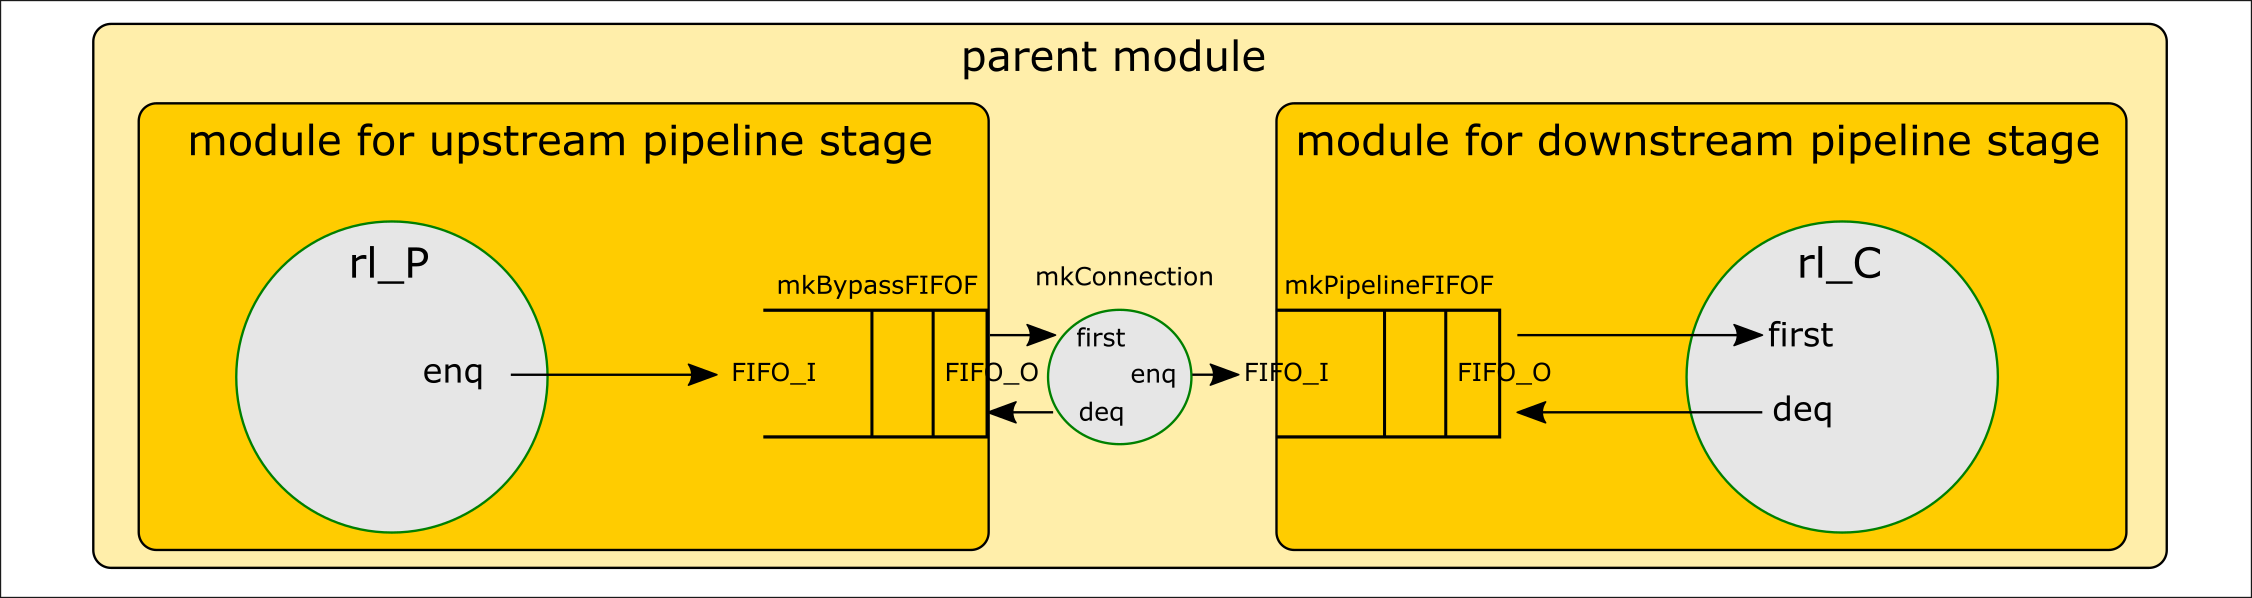
\includegraphics[width=6in,angle=0]{Figures/Fig_Composed_FIFO_modularity}}
  \caption{\label{Fig_Composed_FIFO_modularity_1}
           How we connect Fife stages}
\end{figure}

In the upstream (producer) stage we instantiate a
\verb|mkPipelineFIFOF|.  The rules in the stage enqueue outgoing
information into the \verb|FIFO_I| side of the FIFO using the
\verb|enq| method, and we lift the \verb|FIFO_O| side to the
stage-module interface.

Conversely, in the downstream (consumer) stage we instantiate a
\verb|mkBypassFIFOF|.  The rules in the stage consume incoming
information from the \verb|FIFO_O| side of the FIFO using the
\verb|first| and \verb|deq| methods, and we lift the \verb|FIFO_I|
side to the stage-module interface.

Finally, in the parent module, we use \verb|mkConnection| to connect
the exposed \verb|FIFO_O| and \verb|FIFO_I| ends of the FIFOs.

The benefits of this technique are discussed in
Section~\ref{Sec_SpecialFIFOs}.  Suffice it to say, here, that:

\begin{tightlist}

 \item Despite there being two FIFOs, data can traverse from producer
       to consumer in 1 tick, as desired.

 \item The structure allows the producer and consumer to be compiled
       independently by \emph{bsc}, with no ``rule-scheduling''
       constraints leaking across stage boundaries.

 \item There are no combinational paths crossing the stage boundary
       (through the two FIFOs).

 \item The structure allows us to reason about (and prove) correctness
       of each stage completely independently of other stages.

\end{tightlist}
All of these are pleasing ``modularity'' properties of the design.

% ****************************************************************

\section{Polymorphic and Monomorphic Types}

\label{Sec_Polymorphic_Types}

\index[BSV]{Polymorphic Types}
\index[BSV]{Polymorphic Types!Type variables (identifiers beginning with lower-case letter)}
\index[BSV]{Type variables!Identifiers beginning with lower-case letter, for polymorphism}

\index[BSV]{Monomorphic Types (types without type-variables)}

The previous sections showed several \emph{polymorphic} types:

{\footnotesize
\begin{tightlist}
 \item \verb|Reg #(t)|
 \item \verb|RegFile #(index_type, content_type)|
 \item \verb|GPRs_IFC #(reg_width)|
 \item \verb|FIFOF #(t)|
 \item \verb|FIFOF_I #(t)|
 \item \verb|FIFOF_O #(t)|
\end{tightlist}
}

In each case, there is a \emph{type constructor} ({\tt Reg}, {\tt
RegFile}, ..., {\tt FIFOF\_O}) applied to some arguments ({\tt t},
{\tt ix\_width}, {\tt reg\_width}).  The general syntax is:

\begin{tabbing}
\hmm \emph{type-constructor} {\tt \#(}\emph{arg}, ..., \emph{arg}{\tt )}
\end{tabbing}

(When a type constructor has no arguments, we can omit ``{\tt \#()}''.)

When the argument of a type-constructor is an identifiers beginning
with a lower-case letter, this indicates that this is a \emph{type
variable}, {\ie} it is place-holders for some specific type that will
be instantiated later/elsewhere.

A polymorphic type (a type containing one or more type-variables)
represents all possible types one can obtain by instantiating the type
variables with specific, concrete types.  A type with no
type-variables is also called \emph{monomorphic}.

Note that it is not just library types ({\tt Reg}, {\tt RegFile}, {\tt
FIFOF}) that may be polymorphic.  In the previous sections, we defined
new types \verb|GPRs_IFC #(reg_width)|, \verb|FIFOF_I #(t)| and
\verb|FIFOF_O #(t)| that are also polymorphic.

% ----------------------------------------------------------------

\EXERCISE{Ex-07-B-Polymorphic-Types}

% ================================================================

\subsection{Polymorphic Modules and Synthesizability into Verilog}

\label{Sec_Polymorphic_Types_and_Synthesizability}

\index[BSV]{synthesize@{\tt synthesize}!attribute on modules for Verilog generation}

In Section~\ref{Sec_Module_Definitions} we mentioned without
discussion that the ``{\tt (* synthesize *)}'' attribute preceding a
{\tt module} definition controls whether the \emph{bsc} compiler
generates a Verilog module for this {\BSV} module or whether it is
inlined into its parent module wherever it is instantiated.

Not all {\BSV} modules can be compiled one-to-one into Verilog modules.
Broadly speaking, polymorphic modules cannot be separately compiled
into Verilog modules.  The reason is that polymorphism in {\BSV} is very
powerful and, beyond the expressive power of Verilog.

This does not mean that we cannot use polymorphic modules in a {\BSV}
design; of course we can!  It just means that, at each instance of the
module where we have instantiated it and fully specified the types
(``monomorphized'' the types), the \emph{bsc} compiler at that place
has enough information to generate Verilog for that instance.

For example, consider the polymorphic {\tt mkRISCV\_GPRs} module
Section~\ref{Sec_RISCV_regfile}.  We can directly instantiate this
module in a CPU module:

{\footnotesize
\begin{Verbatim}[frame=single, numbers=left]
module mkCPU;
   ...
   GPRs_IFC #(XLEN) gprs <- mkGPRs;
   ...
endmoduile
\end{Verbatim}
}

At this instantiation position, the \emph{bsc} compiler knows the
concrete value ({\tt XLEN}) of the type-variable {\tt xlen}, and so
can generate Verilog code for this {\tt mkRISCV\_GPRs} instance.  In
the final Verilog code, there will not be any separately identifiable
Verilog code for the register file, it would just be part of the {\tt
mkCPU} module Verilog.

If we really wanted to generate a separately identifiable Verilog
module for the register file, we can write a monomorphic wrapper
module:

{\footnotesize
\begin{Verbatim}[frame=single, numbers=left]
(* synthesize *)
module mkGPRs_V (GPRs_IFC #(XLEN));
   GPRs_IFC #(XLEN) ifc <- mkGPRs;
   return ifc;
endmoduile
\end{Verbatim}
}

This module {\tt mkRISCV\_GPRs\_V} is monomorphic because the
type-variable {\tt xlen} has been instantiated to the concrete type
{\tt XLEN}, and so the ``{\tt (* synthesize *)}'' attribute will be
honored by the \emph{bsc} compiler to produce a corresponding Verilog
module.

We can then replace our earlier instantiation of {\tt mkRISCV\_GPRs}
in the CPU module with this monomorphic module:

{\footnotesize
\begin{Verbatim}[frame=single, numbers=left]
module mkCPU;
   ...
   GPRs_IFC #(XLEN) gprs <- mkGPRs_V;
   ...
endmoduile
\end{Verbatim}
}

% ----------------------------------------------------------------

\EXERCISE{Ex-07-C-Synthesizable-Modules}

% ****************************************************************
